% !TeX root = ./5-handout.tex

%possible excursion topics:
%could also get into the law of nature stuff this week! or save for probability! or even for the last day of class. 
%free will
%causal explN background: e.g. woodward view (could be relevant for time-travel stuff, so could also save for later)
%rationality: straightforwardly factual vs. normative/plan-laden; defs relevant for decision theory unit! and whether dominance reasoning is rational. 

%stuff on axiom of choice: relevant for bacon's puzzle
%could also save bacon puzzle for AoC unit! or return to later 
%could couple w/ Yablo's extension case, where the strategy to Bacon's paradox seems to lead to a genuine contradiction!!! see my notes in 3-thoughts and also the slides he sent me. Bevs vs. Owls 


% could incorporate/do if needing to kill time:
% chalk and talk the review sheet for this week
% talk about the strangeness of reductio proofs (could do this in future as well!); but defs relevant this week given large number of reductio proofs on the pset 
%changes to notion of rigor in mathematics; e.g. bolzano moving away from physical intuition , motion, passage of time. 


%\newcounter{mysection}
%\setcounter{mysection}{1}
%\arabic{mysection}
%\roman{subsection}

%\begin{itemize}[<+->] 
%\item<2-> % reveals second and keeps on page in subsequent frames
%\begin{itemize}[<2->] %does for a whole list of items


\setcounter{section}{4} %sets section counter to 0. note that need to switch section counter from Roman to arabic for this to work! since no roman numeral for 0! %put this into preamble, i.e. file common.tex: \renewcommand\thesection{\arabic{section}}




\section{Decision Theory \& Newcomb}
%\subsection*{test}

\begin{frame}
%\large

\scriptsize{\tableofcontents}

\end{frame}


\begin{frame}
\frametitle{Liable to forget:}
%\large

\begin{itemize}[<+->]

\item PSet 5 is due this Sunday 3/26, 5pm!

\item[] questions 2--5 can be read in Part I quiz component %which i hopefully won't delete this week

\item Spring break starts Monday 3/27! 

\item[] No Pset due Sunday 4/2

\item Feel free to join \href{https://piazza.com/mit/spring2023/24118}{Piazza}! 

\item Feel free to join PSet partners!
\item[] Groups will be auto-assigned Thursday 


\end{itemize}
\end{frame}

\subsection{Newcomb's Problem}

\begin{frame}
\frametitle{An Easy Case (No Predictor)}
%\large

\begin{itemize}[<+->]
\item There are two boxes. The transparent box contains \$1K

\item You don't know what the opaque box contains, 

\item[] but it's either \$0 or \$1 million (\$1M.) You have two choices: 

\item[] \emphz{Two-Box}: Keep both boxes (i.e. acquire their contents)
\item[] \emph{One-Box}: Keep the opaque box; leave the transparent box

\item The boxes were sealed before you entered the room, and your choice will not cause their contents to change. 

\item How should you choose?

\end{itemize}
\end{frame}

\begin{frame}
\frametitle{Newcomb's Problem (with fallible predictor)}
%\large

Same as before, except now the contents of the opaque box were selected by \emph{a predictor}, who is known to be 99\% accurate

\begin{itemize}[<+->]

\item If the predictor predicted you will one-box, they placed \$1M in the opaque box

\item If the predictor predicted you will two-box, they left the opaque box empty

\item Either way, the transparent box has \$1000 (i.e. \$1K)

\item As before, the boxes were sealed before you entered, and your choice cannot cause their contents to change.

\item How should you choose? 

\end{itemize}
\end{frame}

\begin{frame}
\frametitle{Your Value/Utility Function}
%\large

\begin{itemize}[<+->]

\item Throughout this unit, we will assume that you value only money (and value it linearly)

\item You assign value \(n\) to a situation in which you net \(\$n\)

\item There is no diminishing marginal utility (you're tryin to be Jeff Bezos rich)
%``Diminishing marginal utility refers to the phenomenon that each additional unit of gain leads to an ever-smaller increase in subjective value. For example, three bites of candy are better than two bites, but the twentieth bite does not add much to the experience beyond the nineteenth (and could even make it worse).''


\end{itemize}
\end{frame}

\begin{frame}
\frametitle{Philosophy Prompt \#11: Does anyone need a new comb?}
%\large

\begin{itemize}[<+->]

\item You have been placed within a Newcomb's problem with 99\% accurate predictor, and you're hoping to make mad bills \$\$\$

\item Would you \emph{one-box} or \emphz{two-box}, and why? 

\item If the predictor were infallible, would this change your decision? Why or why not?

\end{itemize}

\begin{longtable}[c]{@{}lll@{}}

%& \textit{Contents of} & \textit{the boxes:} \tabularnewline
& \multicolumn{2}{c}{\textit{Contents of each box:}} \tabularnewline
\textbf{Prediction:} & \textit{Opaque Box} & \textit{Transparent Box}
\tabularnewline
\hline
\endhead
\textbf{One-Box} & \emph{\$1M} & \$1K\tabularnewline
\textbf{Two-Box} & \emphz{\$0} & \emphz{\$1K}\tabularnewline
\hline
\end{longtable}

\end{frame}

\begin{frame}
\frametitle{A Quick Case for \emph{One-boxing}}
%\large

\begin{itemize}[<+->]

\item
  {If you one-box, it is almost certain
  (99\%) that the opaque box will contain \$1M;}

\item
  {If you two-box, it is almost certain (99\%)
  that~the opaque box will be empty.
  }


\end{itemize}
\end{frame}

\begin{frame}
\frametitle{A Quick Case for \emphz{Two-boxing}}
%\large

\begin{itemize}[<+->]

\item
  If the opaque box is empty, you'll be better off if you two-box than if you
  one-box.
\item
  If the opaque box is full, you'll be better off if you two-box
  than if you one-box.


\end{itemize}
\end{frame}

\subsection{Decisions Decisions}

\begin{frame}
\frametitle{(Evidential) Decision Theory}
%\large

\fbox{\parbox{135mm}{$$\text{your options} + \text{the probabilities} + \text{your values} \Rightarrow \text{a recommendation}$$}}

\begin{itemize}[<+->]

\item Each \textbf{act} (i.e. choice/option) is associated with various conditional probabilities for different states of affairs obtaining

\item Each state of affairs \& choice has a utility/value to you

\item E.g. You can decide to go to the ice cream shop or not.

\item[] \textit{States of affairs}: shop is open and has your favorite flavor, \\ shop is open but the flavors stink, shop is closed, you get in a traffic accident and never make it; you're safe at home 

\item \emph{Expected Value Maximization}: Choose an option whose \emph{expected value} is at least as high as that of any rival option.\label{gloss:evm}

\end{itemize}
\end{frame}

\begin{frame}
\frametitle{(Evidential) Expected Value}
%\large

The \emph{expected value} of an option $A$ is the weighted average of the value of the outcomes that $A$ might lead to, with weights determined by the probability of the relevant outcome, given that you choose $A$: \label{gloss:ev} 

\pause

\[
EV(A) = v(A S_1) \cdot p(S_1|{}A) + 
 \ldots + 
v(A S_n) \cdot p(S_n|{}A)
\]

\begin{itemize}[<+->]

\item ``$S_1, S_2,\ldots, S_n$'' is any list of (exhaustive and mutually exclusive) states of the world (i.e. outcomes);

\item ``$v(A S_i)$'' is the value of being in a situation in which you've chosen $A$ and state $S_i$ is the case;

\item ``$p(S|A)$'' is the probability of $S$, given that you choose $A$.\label{gloss:cond-prob5}


\end{itemize}
\end{frame}

\begin{frame}
\frametitle{Illustration: Newcomb's Problem}
%\large

\begin{itemize}[<+->]

\item Exhaustive and mutually exclusive states of affairs: 
\item[] $F$: the opaque box is full 

\item[] $E$: the opaque box is empty

\item \textit{Acts/options/choices}: ``$1$'': you select only the opaque box 

\item[] ``$2$'': you select both boxes

\item \textit{Values}: $v(1 F) = 1M$; $v(1 E) = 0$

\item[] $v(2 F) = 1.001M$; $v(2 E) = 1K$


\end{itemize}
\end{frame}

\begin{frame}
\frametitle{Calculating EVs in Newcomb's problem}
%\large

\begin{itemize}[<+->]

\item Let's calculate the expected values of one-boxing vs. two-boxing

\item For the PSet Part 2: write the equations in abstract form, substitute numerical values, and calculate step-by-step: 

\[
\begin{array}{ccc}
EV(1) &= &v(1\, F) \cdot p(F|1) + v(1\,E) \cdot p(E|1)\\ \pause 
 &= &1M  \cdot 0.99 + 0 \cdot 0.01 \\ \pause 
 &= & 990,000 \\  \pause 
 & & \\ \pause 
EV(2) &= &v(2\, F) \cdot p(F|2) + v(2\,E) \cdot p(E|2)\\ \pause 
 &= &1.001M  \cdot 0.01 + 1K \cdot 0.99 \\ \pause 
 &= & 10,010 + 990 = 11,000 \\ 
\end{array}
\]

\item So EV Maximization recommends one-boxing

\item Is this the right result????

\end{itemize}
\end{frame}

\subsection{If I tell you, I'll have to \dots}

\begin{frame}
\frametitle{Indicative vs. Subjunctive Conditionals}
%\large

Past Events: \\ \textit{Context}: LH Oswald assassinated JFK on 11/22/1963; he acted alone 
\pause
\begin{quote}
\begin{description}
\item[Indicative] If Oswald didn't shoot JFK, someone else did. \pause
\item[Subjunct.] Had Oswald not shot JFK, someone else would have (this is a ``counterfactual''!) \pause
\end{description}
\end{quote}

Present Events:
\begin{quote}
\begin{description}
\item[Indicative] If people are using their umbrellas, it's raining.\pause
\item[Subjunctive] Were people to use their umbrellas, there would be rain. (make it rain!!!)\pause


\end{description}
\end{quote}



\begin{quote}
\begin{description}
\item[Indicative] If it's raining, people are using their umbrellas.\pause

\item[Subj.] Were it to rain, people would use their umbrellas.

\end{description}
\end{quote}
\end{frame}

\begin{frame}
\frametitle{Indicative Conditionals}
%\large

\begin{itemize}[<+->]

\item ``$A \rightarrow B$'' is shorthand for the indicative conditional``if $A$, then $B$''.


\item The probability of an indicative conditional is the conditional probability of its consequent given its antecedent:\footnote{Provided that $A$ contains no indicative conditionals.}
$$p(A \rightarrow B) = p(B|A)$$

\item So we can re-express (evidential) expected utility in terms of indicative conditionals \pause
\end{itemize} 

\[
\begin{array}{ccc}
EV(A) &= &v(A S_1) \cdot p(S_1|{}A) + \ldots + v(A S_n) \cdot p(S_n|{}A)\\ \pause 
& = & v(A S_1) \cdot p(A \rightarrow S_1) + \ldots + v(A S_n) \cdot p(A \rightarrow S_n)
\end{array}
\]


\end{frame}

\begin{frame}
\frametitle{Subjunctive Conditionals: They're for a Good Cause}
%\large

\begin{itemize}[<+->]
\item ``$A \must B$'' is shorthand for the subjunctive conditional \\ ``If it were the case that $A$, then it would be the case that $B$''

\item If $A$ causes $B$, then, typically, $A \must B$. 

\textbf{Example}: Rain causes people to use their umbrellas. \\ So: were it to rain, people would bust out their umbrellas.

\item Bob Stalnaker provided a semantics for these in 1968 \\ (we missed Stalnaker's b-day on Jan 22!) 



\end{itemize}
\end{frame}

\begin{frame}
\frametitle{Subjunctives for No Cause}
%\large

\begin{itemize}[<+->]

\item If $A$ doesn't cause $B$, then, typically the following are true:
\begin{itemize}

\item If $B$: $A \must B$ and $\neg A \must B$; or

\item If $\neg B$: $A \must \neg B$ and $\neg A \must \neg B$

\end{itemize}

\item \textbf{Example}: Umbrella use doesn't cause rain. Assuming it's sunny:

%\begin{description}
\item[] Were people to use their umbrellas, it would (still) be sunny \\[1ex] \makebox[\textwidth]{and}
\item[] Were people to not use their umbrellas, it would (still) be sunny% outside.
%\end{description}
\end{itemize}
\end{frame}

\subsection{Causal Decision Theory}

\begin{frame}
  \frametitle{Happy Birthday to Benardete tomorrow!}

  \begin{columns}
    \begin{column}{.35\textwidth}
      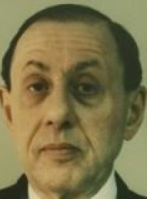
\includegraphics[height=.6\textheight]{../assets/Benardete_photo}
    \end{column}
    \begin{column}{.7\textwidth}
      \begin{itemize}[<+->]
        \item Jos{\'e} Benardete (1928--2016)
        
        %taught at syracuse from 1961 onwards! so for over 50 years
        
        \item Metaphysician and historian of Early Modern philosophy 
        
        \item Namesake for Benardete's paradox!
        
        \item[] -- A reverse omega sequence of Gods stand ready to raise their barrier iff no early God has raised their barrier
        \item[] -- What stops you from passing through Gods?
        %basically founded set theory! 
      \end{itemize}
    \end{column}
  \end{columns}
\end{frame}

\begin{frame}
\frametitle{Causal Decision Theory: ECU}
%\large

\begin{itemize}[<+->]

\item \emphz{Expected causal utility} (ECU) of an option $A$: the weighted average of the values of $A$'s possible outcomes, with weights determined by the probability of the following subjunctive conditional: \textit{were you to perform} $A$, \textit{the outcome would obtain}. 
\end{itemize}
\pause 
\[
\hspace{-1em} ECU(A) = v(A S_1) \cdot p(A \must S_1) +  v(A S_2) \cdot p(A \must S_2) + \ldots +  v(A S_n) \cdot p(A \must S_n)
\]

\begin{itemize}[<+->]

\item ``$S_1, S_2,\ldots, S_n$'' is any list of (exhaustive and mutually exclusive) states of the world (i.e. outcomes);

\item ``$v(A S_i)$'' is the value of being in a situation in which you've chosen $A$ and state $S_i$ is the case;

\item ``$p(A \must S)$'' is (roughly) the probability that act $A$ brings about $S$\label{gloss:cond-prob6}
%i should get a better gloss on this probability; think about more. see the SEP page for causal decision theory for help! 
% obtains, given that you choose $A$.


\end{itemize}
\end{frame}

\begin{frame}
\frametitle{Causal Decision Theory: Max ECU}
%\large

\[
\hspace{-1em} ECU(A) = v(A S_1) \cdot p(A \must S_1) +  v(A S_2) \cdot p(A \must S_2) + \ldots +  v(A S_n) \cdot p(A \must S_n)
\]

\begin{itemize}[<+->]

\item \emphz{Expected Causal Utility Maximization}: In any decision problem, you ought to choose an option whose expected causal utility is at least as high as that of any rival option. 

\item In the \textbf{special case} where each $S_i$ ($i \leq n$) is a state of affairs whose obtaining or not is causally independent of action $A$, ``$A \must S_i$'' is equivalent to ``$S_i$''. 

\item[] This yields:
\[
ECU(A) = v(A S_1) \cdot p(S_1) +  v(A S_2) \cdot p(S_2) + \ldots +  v(A S_n) \cdot p(S_n)
\]

\end{itemize}

\end{frame}

\begin{frame}
\frametitle{Illustration: Newcomb's Problem}
%\large

Recall that for Newcomb's Problem, we have:

\begin{itemize}%[<+->]

\item Exhaustive and mutually exclusive states of affairs: 
\item[] $F$: the opaque box is full 

\item[] $E$: the opaque box is empty

\item \textit{Acts/options}: ``$1$'': you select only the opaque box 

\item[] ``$2$'': you select both boxes

\item \textit{Values}: $v(1 F) = 1M$; $v(1 E) = 0$

\item[] $v(2 F) = 1.001M$; $v(2 E) = 1K$


\end{itemize}
\end{frame}

\begin{frame}
\frametitle{Calculating ECUs in Newcomb's problem}
%\large

\begin{itemize}[<+->]

\item Calculate the expected causal utilities of 1-boxing vs. 2-boxing: 

\item Key fact: since the contents of the boxes are causally independent of your decision, the probabilities of the subjunctive conditionals equals the probability of the different outcomes:

\item[] $p(1 \must  F) = p(F)$, $p(2 \must  F) = p(F)$, etc. 

%\item For the PSet Part 2: write the equations in abstract form, substitute numerical values, and calculate step-by-step: 

\[
\begin{array}{ccc}
ECU(1) &= &v(1\, F) \cdot p(1 \must F) + v(1\,E) \cdot p(1 \must E)\\ \pause 
&= &v(1\, F) \cdot p(F) + v(1\,E) \cdot p(E)\\ \pause 
 %&= &1M  \cdot 0.99 + 0 \cdot 0.01 \\ \pause 
% &= & 990,000 \\  \pause 
 & & \\ \pause 
ECU(2) &= &v(2\, F) \cdot p(2 \must F) + v(2\,E) \cdot p(2 \must E)\\ \pause 
 &= &v(2\, F) \cdot p(F) + v(2\,E) \cdot p(E)\\ \pause
% &= &1.001M  \cdot 0.01 + 1K \cdot 0.99 \\ \pause 
% &= & 10,010 + 990 = 11,000 \\ 
\end{array}
\]

\item Since, $v(2\, F) > v(1\, F)$ and $v(2\, E) > v(1\, E)$: $ECU(1) < ECU(2)$

\item So ECU Maximization recommends two-boxing!

%\item Have we saved the day?

\end{itemize}
\end{frame}

\subsection{Being for two-boxing}

\begin{frame}
\frametitle{Strongly Dominant Strategies}
%\large

\begin{itemize}[<+->]

\item A strategy or act/option $A$ \emphz{strongly dominates} rival acts iff no matter the outcome, you are better off choosing $A$ over any rival 

\item If the opaque box is empty, you are better off two-boxing: \\ \$1K rather than \$0

\item If the opaque box is full, you are better off two-boxing: extra \$1K

\item So no matter what, you are better off two-boxing

\end{itemize}
\end{frame}

\begin{frame}
\frametitle{Dominance as a Principle of Rationality}
%\large

\begin{itemize}[<+->]

\item \emphz{Dominance}: if an act $A$ strongly dominates, then you \textit{ought} to choose $A$

\item[] -- If you do not choose $A$, then you are \textcolor{red}{irrational} 

\item Note that if any of your friends were able to see into the opaque box, then no matter what, they would recommend two-boxing. 

\item If you one-boxed, it would seem to your friend that you are leaving money on the table, which seems irrational

\end{itemize}
\end{frame}

\subsection{Being for one-boxing}

\begin{frame}
\frametitle{Infallible Predictor}
%\large

\begin{itemize}[<+->]

\item Consider the case of an infallible predictor: \\ 100\% accurate, not just in the past but for all time 

\item It seems that there are only two \textit{possibilities}: \\ (i) you one-box and get \$1M x-or (ii) you two-box and get \$1K

\item If rationality requires 1-boxing here, then if you endorse the following principle, you'll endorse 1-boxing in the fallible case 

%\item Like being able to affect the past but not change it: if you are determined to one-box then you're determined to get rich. but you still have to one-box! 
%perhaps the two-boxer is a kind of fatalist: thinking that they will fail to be rich no matter what they do. for i assert that had they one-boxed, then they would have been rich. but note how this is a backtracking cF. 
%i appreicate how agustin in the video notes that we're really at brass tacks/temperament on the question of whether back tracking cFs are appropriate in this case. 

\item \emph{Recommendation Continuity}: The recommendations of a decision theory should not change discontinuously as probabilities of outcomes change continuously
%%but issue w/ this principle: the acts are discontinuous. only mixed strategies of these acts could vary continuously...so more precisely, if a decision theory recommends 1-boxing 100\% of the time in infallible case, then it ought to recommend 1-boxing arbitrarily close to 100\% of the time as we introduce a small chance of fallibility. 

\item Hence, if we introduce a small chance $\epsilon$ of the predictor making an error, our decision theory should yield an arbitrarily close/similar recommendation in the case of $(100-\epsilon)\% $ accuracy 

\end{itemize}
\end{frame}

\subsection{Rationality!}

\begin{frame}
\frametitle{Philosophy Prompt \#12: Let's try to be rational}
%\large

\begin{enumerate}[<+->]

\item Are you necessarily \textcolor{red}{irrational} if you violate \emphz{Dominance} \\ (e.g. by choosing to 1-box in a Newcomb's problem)?
\item[] i.e. is it ever rationally permissible to choose a strongly dominated option? 

\item Are you necessarily \textcolor{red}{irrational} if you violate \emph{Recommendation Continuity} (e.g. by endorsing 1-boxing in the infallible case but 2-boxing otherwise)?

\item What is the status of these claims about ``rationality'' anyways? e.g. are rationality facts like facts about the positions of tables, facts about numbers, facts about morality, \dots?

\end{enumerate}
\end{frame}

\begin{frame}
\frametitle{Descriptive vs. Non-descriptive Claims}
%\large

\begin{itemize}[<+->]

\item \emphz{Descriptive claim}: purports to mirror or represent the way the world is, i.e. some state of affairs

\item[] e.g. ``There is a chalkboard behind me and in front of you''

\item \emph{Non-descriptive claim}: Performs some non-representational functional role

\item[] e.g. expresses an attitude or command

\item[] e.g. ``don't be late''! 

\end{itemize}
\end{frame}


\begin{frame}
\frametitle{To be continued! }
%\large

\begin{itemize}[<+->]

\item We will continue this discussion of the nature of rationality at some point in a future topic!

\item Likewise, we'll return to free will! Still lots of good stuff to discuss! 

\item After break, we start a unit on probability, and then we move into some measure theory and issues surrounding the Axiom of Choice

\end{itemize}
\end{frame}


\iffalse %*********************************************************************

\begin{frame}
\frametitle{Moral Expressivism}
%\large

\begin{itemize}[<+->]

\item \emph{Moral Expressivism}: moral claims are non-descriptive; specifically they express pro- or con- attitudes toward various actions

\item ``The right thing to do is to hold the door open for people'': expresses an attitude of

\item[]  \textit{being for holding the door open for others} 

\item Alternatively: expresses acceptance of a set of norms that \textit{recommend} (or at least permit) holding the door open for others

\end{itemize}
\end{frame}

\begin{frame}
\frametitle{Expressivism about Rationality (Gibbard 1990)}
%\large

\begin{itemize}[<+->]

\item To judge that an action is rational is to express acceptance of a set of norms that recommend (or at least permit) that action

\item To judge that an action is irrational is to express acceptance of a set of norms that forbid that action

\item For every action, a complete set of norms renders it required, recommended, permissible, or forbidden 

\item We need not think that judgments of rationality are ``straightforwardly factual'' (they need not be tracking or mirroring states of affairs); they can remain factual in a weaker, more deflationary sense 

%thinking what you ought to do is thinking what to do

\end{itemize}
\end{frame}

\begin{frame}
\frametitle{On the Rationality of \emphz{Dominance}}
%\large

\begin{itemize}[<+->]

\item Proponents and opponents of \emphz{Dominance} are at least in a normative dispute:

\item[] They disagree about the norms we ought to endorse when it comes to making decisions

\item Proponents of \emphz{Dominance} are always in favor of choosing strongly dominant strategies

\item Opponents believe that we ought to allow for exceptions 

\item What could settle who is ultimately right? 

\item[] -- i.e. what settles what we should do?


\end{itemize}
\end{frame}

\subsection{Free Willy!}

\begin{frame}
\frametitle{Surface Free Will (just superficial enough)}
%\large

\begin{itemize}[<+->]

\item \emph{Surface free will} (a.k.a. compatibilist free will or political free will): the political or social ability to make choices that satisfy your desires. The freedom to do what you want to do.
\item Perhaps the ordinary or intuitive notion of freedom of choice/will
\item A power or ability to choose something rather than something else
\item ``unconstrained freedom of choice or decision'' [Kane, p. 15], \\ coming from within you

\item as in, \textit{Reach for the stars, not drugs} 

\end{itemize}
\end{frame}

\begin{frame}
\frametitle{Libertarian Free Will (it's apolitical!)}
%\large

\begin{itemize}[<+->]

\item \emphz{Libertarian Free Will}: (a.k.a.` free will of origination'): 
\item[] -- the ability to choose what you \textit{want to want} or want to desire. 
\item Having ultimate power over what you will/want/desire. %Kane refers to this as a deeper sense of free will
\item ``a kind of ultimate control over what you will or want in the first place'' [Kane, p. 15]

\item The kind of free will your soul craves 


\end{itemize}
\end{frame}

\begin{frame}
\frametitle{Compatibilism vs. Incompatibilism}
%\large

\begin{itemize}[<+->]

\item \textbf{Compatibility Question}: is free will compatible with determinism? Likewise, is free will compatible with any physically-plausible version of indeterminism?

\item If you answer `yes,' then you are a \emph{compatibilist}
\item[] -- \textit{soft determinist}: you also believe determinism is true 

\item If you answer `no,' then you are an \emphz{incompatibilist}: 

\item \textit{hard determinist}: you also believe that determinism is true
\item[] -- so you deny we have the relevant kind of free will

\item \textit{libertarian} (about free will): you also deny determinism
\item[] -- so you believe we do have free will (modulo worries about compatibility with indeterminism!)

\end{itemize}
\end{frame}

\begin{frame}
\frametitle{(Classical) Compatibilism}
%\large

\begin{itemize}[<+->]

%\item free will has one necessary and sufficient condition: 

\item (Classical) \emph{Compatibilism}: you acted freely if and only if you met the following condition: 

\item \textbf{Weak Principle of Alternative Possibilities}: if you had wanted to choose otherwise than you did, then nothing would have prevented you from choosing otherwise.
%Frankfurt cases provide a counterexample to the necessity of this condition. still seems sufficient though. 

\item Notice that meeting this condition entails that another claim holds: you have the power or ability to make a choice in the sense that nothing constrains you or prevents you from making that choice

\item According to compatibilism, a sufficient condition for LACKING free will in a given circumstance is that you are constrained, coerced, or otherwise manipulated


%\item Hence, if anything does constrain you or prevent you from making that choice, then you don’t have this power or ability to do what you want to do, and hence you could not have chosen otherwise. 

\end{itemize}
\end{frame}

\begin{frame}
\frametitle{Compatibility with Moral Responsibility}
%\large

\begin{itemize}[<+->]

\item Imagine that you don't think free will is necessary for moral responsibility: e.g. an agent can be morally responsible for their actions even if they did not act freely 
\item[] -- roughly, you think it would still be appropriate to praise or blame this agent for their action

\item You might then ask a similar `compatibility question' about whether moral responsibility is compatible with determinism

\item e.g. perhaps \textit{surface free will} suffices for moral responsibility 

\item When it comes to social and political decisions, you might think that moral responsibility is really what matters 

\end{itemize}
\end{frame}


\fi %*********************************************************************